\documentclass[12pt]{article}
\usepackage{CJKutf8}
\usepackage{geometry}
\usepackage{listings}
\usepackage{amsmath}
\usepackage{commath}
\usepackage{graphicx}

\lstset{frame=tb,
    language=Matlab}

\newgeometry{vmargin={6mm,10mm}, hmargin={10mm,10mm}}   
\begin{CJK}{UTF8}{bsmi}
\author{b05502087 王竑睿}
\date{}
\title{數值線性代數 HW3}

\begin{document}
\maketitle
\section{Consider the basic iterative method}
$$Mx_{k+1} = Nx_k + b$$
\subsection{(a) Show that the spectral radius of $G = M^{-1}N$ approximately satisfies $$\rho(G) \approx \dfrac{x_{k+1}-x_{k}}{x_{k}-x_{k-1}}$$}
    \[
        \begin{aligned}
            &x_{k+1}=Gx_k+M^{-1}b\\
            &x_{k}=Gx_{k-1}+M^{-1}b\\
        \Rightarrow &x_{k+1}-x_{k}=G(x_k-x_{k-1})\\
        \Rightarrow &y_{k}=Gy_{k-1} \quad \text{(令$y_k=x_{k+1}-x_{k}$)}\\
        \end{aligned}
    \]
    \text{藉由 power method, }\\
    \text{知道 $y_{k-1}$ 會趨近於dominant eigenvector y}\\
    \[
        \begin{aligned}
        \Rightarrow &y_{k}=Gy_{k-1} \approx Gy = \lambda y \approx \lambda y_{k-1}\\
        \Rightarrow &\dfrac{\norm{y_{k}}}{\norm{y_{k-1}}} \approx \abs{\lambda} = \rho(G)\\
        \Rightarrow &\rho(G) \approx \dfrac{\norm{x_{k+1}-x_{k}}}{\norm{x_{k}-x_{k-1}}}\\
        \end{aligned}
    \]    
\subsection{(b) Show that if $\rho(M^{-1}N)$ is known, an estimate for the error is given by
                $$\norm{x_k - x}_2 \leq \dfrac{\rho(G)}{1-\rho(G)}\norm{x_k - x_{k-1}}_2$$
            }

        先證明 $\norm{e_{k+1}}_2 \leq \rho(G)\norm{e_{k}}_2$
    \[
        \begin{aligned}
            &x_{k+1}=M^{-1}(b+Nx_k)\\
\Rightarrow &x_{k+1}=x_{k}+M^{-1}(b-Ax_k) \quad \text{(A=M-N)}\\
\Rightarrow &e_{k+1}=x-x_{k+1} = (x-x_{k})-M^{-1}(b-Ax_k)\\
\Rightarrow &e_{k+1}=(x-x_{k})-M^{-1}A(x-x_k)\\
\Rightarrow &e_{k+1}=(I-M^{-1}A)(x-x_k)\\
\Rightarrow &e_{k+1}=(I-M^{-1}(M-N))e_k\\
\Rightarrow &e_{k+1}=M^{-1}Ne_k\\
\Rightarrow &\norm{e_{k+1}}_2=\norm{M^{-1}Ne_k}_2\leq\norm{M^{-1}N}_2\norm{e_k}_2\\
\Rightarrow &\norm{e_{k+1}}_2\leq \rho{(M^{-1}N)}\norm{e_k}_2 \quad \text{(matrix spectral radius is less than norm)}\\
        \end{aligned}    
    \]
    由題目,令$G=M^{-1}N$\\
    \[
        \begin{aligned}
            &\norm{e_{k}}_2\leq \rho{(G)}\norm{e_{k-1}}_2\\
\Rightarrow &\norm{x-x_k}_2\leq \rho{(G)}\norm{x-x_{k-1}}_2\\
\Rightarrow &\norm{x-x_k}_2\leq \rho{(G)}(\norm{x-x_k}_2+\norm{x_k-x_{k-1}}_2) \quad \text{(三角不等式)}\\
\Rightarrow &\norm{x-x_k}_2\leq \frac{\rho{(G)}}{1-\rho{(G)}}(\norm{x_k-x_{k-1}}_2)\\
\Rightarrow &\norm{x_k-x}_2\leq \frac{\rho{(G)}}{1-\rho{(G)}}(\norm{x_k-x_{k-1}}_2)\\
        \end{aligned}    
    \]

\section{Consider a 500 x 500 sparse matrix A constructed as described in Trefethen and Bau's
book on P. 300.}
利用以下code,產生A,b
\begin{lstlisting}
    function [A,b] = genA(m,n,t)
    % 1 at diagonal
    % random [-1,1] at each off-diagonal (symmtric)
    % each off-diagonal if abs()>t become zero
    A = zeros(m,n);
    for i = 1:m
        for j = 1:i
            if(i==j)
                A(i,j) = 1;
            else
                putIn = (-1+2*rand(1,1));
                if(abs(putIn)>t)
                    A(i,j) = 0;
                    A(j,i) = 0;
                else
                    A(i,j) = putIn;
                    A(j,i) = putIn;
                end
            end
        end
    end
    b = -1+2*rand(m,1);
    %b = rand(m,1);
end
\end{lstlisting}
\subsection{(a) Reproduce Fig.38.1 (the CG convergence curves for this matrix) shown at P.}
利用以下code,進行conjugate gradient method
\begin{lstlisting}
function [X,Y,x,r]=CG(A,b,N)
    [m,n] = size(A);
    Alpha = zeros(1,N+1); %20 iteration
    Beta = zeros(1,N+1); %20 iteration
    r = zeros(m,N+1); %20 iteration residual
    p = zeros(m,N+1); %20 iteration
    x = zeros(n,N+1); %20 iteration

    x(:,1)=zeros(n,1);
    r(:,1)=b; %m
    p(:,1)=r(:,1);

    X = [1:N+1];
    Y = zeros(1,N+1);
    Y(1,1) = norm(r(:,1),2);
    for i=2:N+1
        Aup = r(:,i-1)'*r(:,i-1);
        Adown = p(:,i-1)'*A*p(:,i-1);
        Alpha(1,i) = Aup/Adown;
        
        x(:,i) = x(:,i-1)+Alpha(1,i)*p(:,i-1);

        r(:,i) = r(:,i-1)-Alpha(1,i)*A*p(:,i-1);

        Bup = r(:,i)'*r(:,i);
        Bdown = r(:,i-1)'*r(:,i-1);
        Beta(1,i) = Bup/Bdown;

        p(:,i) = r(:,i)+Beta(1,i)*p(:,i-1);
        norm(r(:,i),2)
        
        Y(1,i) = norm(A*x(:,i)-b,2);
    end
    %norm(r(:,N+1),2)
end
\end{lstlisting}
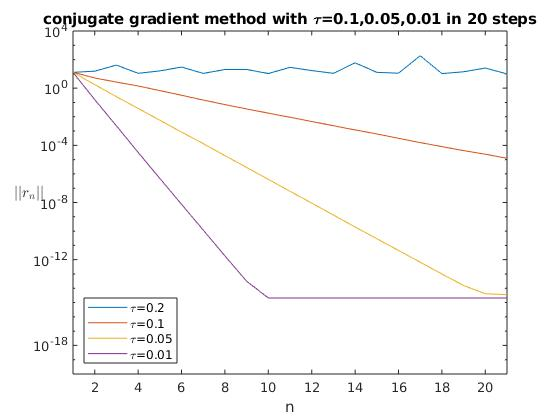
\includegraphics[scale=1]{1.jpg}

\subsection{(b) Produce a plot for $\tau$ = 0.01, 0.05, 0.1
indicating how closely the above estimates match the actual convergence rate}
利用以下code, 計算 convergence rate 以及 error estimate
\begin{lstlisting}
function [X,Y,Y2]=condition(A,b,N,xCG)
    [m,n] = size(A);
    %kappa = norm(inv(A),2)*norm(A,2);
    %using eigenvalue to get kappa
    [V,D]=eig(A);
    lambda_max = max(max(diag(D)));
    lambda_min = min(min(diag(D)));
    kappa = lambda_max/lambda_min;

    xT = A\b;
    %norm(A*xT-b,2)
    e = zeros(m,N+1);

    e(:,1) = xT-xCG(:,1);
    e1A = sqrt(e(:,1)'*A*e(:,1))
    
    X = [1:N+1];
    Y = zeros(1,N+1);
    Y2 = zeros(1,N+1);
    Y(1,1) = 1;
    Y2(1,1) = 1;
    for i=2:N+1
        e(:,i) = xT-xCG(:,i);
        eiA = sqrt(e(:,i)'*A*e(:,i));
        ratio = eiA / e1A;
        bound = 2*(((sqrt(kappa)-1)/(sqrt(kappa)+1))^(i-1));
        %[ratio,bound]
        Y(1,i) = ratio;
        Y2(1,i) = bound;
    end
end
\end{lstlisting}
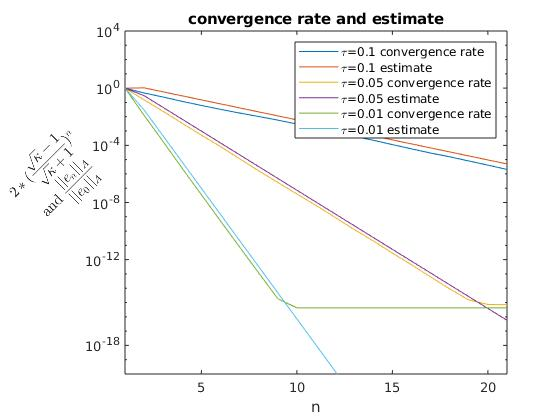
\includegraphics[scale=1]{2.jpg}
\begin{itemize}
    \item 由圖可知,在收斂前,conjugate-gradient method的convergence rate確實會以此estimate為upper bound\\
          且兩者的值相當接近
\end{itemize}

\subsection{(c) Use the method of steepest descent to solve this linear system again and
compare results with those obtained using CG.}
利用以下code, 進行steepest descent method
\begin{lstlisting}
function [X,Y,x,r]=steepest(A,b,N)
    [m,n] = size(A);
    Alpha = zeros(1,N+1); %20 iteration
    r = zeros(m,N+1); %20 iteration residual
    x = zeros(n,N+1); %20 iteration

    x(:,1)=zeros(n,1);
    r(:,1)=b; %m

    X = [1:N+1];
    Y = zeros(1,N+1);
    Y(1,1) = norm(r(:,1),2);
    for i=2:N+1
        Aup = r(:,i-1)'*r(:,i-1);
        Adown = r(:,i-1)'*A*r(:,i-1);
        Alpha(1,i) = Aup/Adown;
        
        x(:,i) = x(:,i-1)+Alpha(1,i)*r(:,i-1);
        r(:,i) = r(:,i-1)-Alpha(1,i)*(A*r(:,i-1)); %steepest

        Y(1,i) = norm(A*x(:,i)-b,2);
    end
end    
\end{lstlisting}
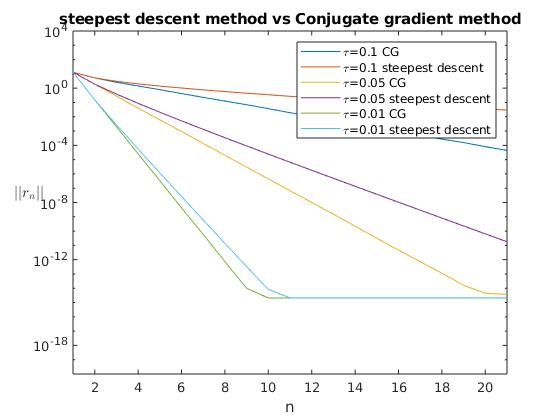
\includegraphics[scale=1]{3.jpg}
\begin{itemize}
    \item 由圖可知steepest descent method的收斂速度較conjugate gradient method慢
\end{itemize}

\subsection{(d) Redo this problem also using the preconditioned conjugate-gradient method
with the gauss-Seidel preconditioner M = D+L. Comments on your results.}
利用以下code, 進行 preconditioned conjugate-gradient method with gauss-Seidel preconditioner
\begin{lstlisting}
%% Solution of x in Ax=b using Gauss Seidel Method
function [X,Y,x]=Precondlib(A,b,tol,maxIt)
    [m,n] = size(A);
    x=zeros(n,1);
    n=size(x,1);
    normVal=Inf; 
    iter = 1;
    Y = [norm(A*x(:)-b,2)];
    while (normVal>tol || iter<=maxIt)
        x_old=x;    
        for i=1:n
            sigma=0;
            for j=1:i-1
                sigma=sigma+A(i,j)*x(j);
            end
            for j=i+1:n
                sigma=sigma+A(i,j)*x_old(j);
            end
            x(i)=(1/A(i,i))*(b(i)-sigma);
        end
        normVal=norm(x_old-x);
        iter = iter + 1;
        Y=[Y,norm(A*x(:)-b,2)];
    end
    X = [1:iter];
end
\end{lstlisting}
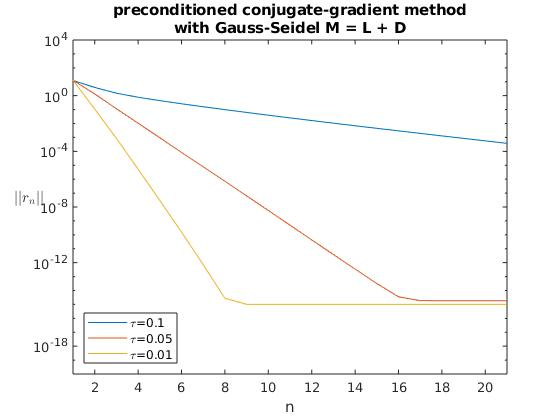
\includegraphics[scale=1]{4.jpg}
\begin{itemize}
    \item 由圖可知,preconditioned conjugate-gradient method的收斂速度較快
    \item $\tau=0.01$時,可利用preconditioned matrix提前2個iteration收斂
    \item $\tau=0.05$時,可利用preconditioned matrix提前4個iteration收斂
\end{itemize}

\end{CJK}
\end{document}